\documentclass[a4paper,openright,12pt]{report}
\usepackage[spanish,activeacute]{babel} % espanol
\usepackage[a4paper,margin=2cm]{geometry} % margenes
\usepackage[latin1]{inputenc} % acentos sin codigo
\usepackage{graphicx} % graficos
\usepackage{amsfonts}
\usepackage{float}
\usepackage{amsmath,amssymb,latexsym,stmaryrd}
\numberwithin{equation}{section} % para numerar ecuaciones
\usepackage{fix-cm}
\usepackage{anyfontsize}
\newtheorem{teorema}{Teorema}[section] % para añadir teoremas
\newtheorem{proposicion}{Proposicion}[section] % para añadir proposiciones
\newtheorem{corolario}{Corolario}[section] % para añadir corolarios
\newtheorem{definicion}{Definicion}[section] % para añadir definiciones
\newtheorem{ejemplo}{Ejemplo}[section] % para añadir ejemplos
\newenvironment{proof}{\noindent{\it Demostracion:}}{\hfill$\blacksquare$} % para las demostraciones, con cuadrado negro al final
\begin{document}
%%%%%% Portada
%\begin{titlepage}

%\begin{center}
%\vspace*{0.6in}
%\begin{figure}[htb]
%\begin{center}
%
\includegraphics[width=8cm]{./logo_uned.png}
%\end{center}
%\end{figure}

%\begin{large}
%TRABAJO FIN DE GRADO.\\
%GRADO EN CIENCIAS MATEM'ATICAS.\\
%\end{large}
%\vspace*{0.15in}
%DEPARTAMENTO DE MATEM'ATICAS FUNDAMENTALES. \\
%\vspace*{0.4in}

%\begin{Large}
%\textbf{REPRESENTACI'ON DE GRUPOS FINITOS.} \\
%\end{Large}
%\vspace*{0.3in}

%\rule{80mm}{0.1mm}\\
%\vspace*{0.1in}
%\begin{large}
%Alumno: \\
%Angel Blasco Mu\~noz \\
%\end{large}

%\rule{80mm}{0.1mm}\\
%\vspace*{0.1in}
%\begin{large}
%Tutor:\\
%Dr. Javier Perez Alvarez\\
%\end{large}
%\rule{80mm}{0.1mm}\\

%\end{center}
%\vspace*{1in}
%\begin{flushright}
%Curso 2018 - 2019
%\end{flushright}
%\end{titlepage}
%%%%%%%%%
%Introduccion de pagina en blanco
%\newpage
%$\ $
%\thispagestyle{empty}
%
%%%% Agradecimientos e indice
\addtocontents{toc}{\hspace{-7.5mm} \textbf{Capitulos}}
\addtocontents{toc}{\hfill \textbf{Pagina} \par}
\addtocontents{toc}{\vspace{-2mm} \hspace{-7.5mm} \hrule \par}

%\chapter*{}
\pagenumbering{Roman} % para comenzar la numeracion de paginas en numeros romanos
%\begin{flushright}
%\textit{A Mateo, mi hijo, \\
%por ense\~narme que lo imposible solo tarda un poco mas.\\
%A Bego\~na, mi mujer, \\
%por toda la paciencia que tiene conmigo.\\
%A Angel y Juliana, mis padres, \\
%por todas las oportunidades que me han dado, incluso cuando no las he %merecido.}
%\end{flushright}
%\chapter*{Agradecimientos} 
%Aqu'i los agradecimientos.
%\begin{abstract}
%Este trabajo versa sobre los grupos finitos y sus representaciones. Es importante destacar que en todo el trabajo al referirnos a \textit{grupo} nos referimos a un  \textbf{conjunto finito} en el cual se definir'a una operaci'on que debe cumplir unos condicionantes, al igual que en los grupos algebraicos propiamente dichos. En los grupos finitos se deben cumplir y respetar las mismas propiedades que en los grupos en general.\\
%\\
%Se introducir'a el concepto de representaci'on de un grupo finito, haciendo especial 'enfasis en el concepto de irreducibilidad, asi como en la teor'ia de caracteres para la determinaci'on de todas las representaciones irreducibles de un grupo dado. Se definir'a a su vez la matriz de caracteres y se calcular'an las representaciones irreducibles de algunos grupos finitos. 
%\end{abstract}
\pagenumbering{arabic} % para comenzar la numeracion de paginas en numeros arabigos
%%% El documento se escribe a partir de aqui en cada chapter, section, etc
%\tableofcontents
%%% Capitulo 1
\chapter{Conceptos b'asicos.}
\section{Grupos.}
Comencemos por definir el concepto de grupo:
\begin{definicion}
Un grupo es un conjunto no vacio G en el que est'a definida una operaci'on que toma dos elementos $a,b \in G$ y nos devuelve otro elemento $ab \in G$
 \[G \times G \rightarrow G \]
que escribiremos \[ (a,b) \mapsto ab \]
tal que:
\begin{enumerate}
\item \textit{(ab)c} = \textit{a(bc)} para cada terna de elementos $a,b$ y $c$ de $G$. Se dice que la operaci'on es \textit{asociativa}.
\item Existe un elemento $u \in G$ tal que \[ua =a=au\] para todos los elementos $a$ de $G$. A este elemento le llamaremos \textit{elemento neutro o elemento identidad}.
\item Para cada elemento $a \in G$ existe $x \in G$ tal que \[ax=u=xa\] A este elemento le llamaremos \textit{inverso} de $a$.
\end{enumerate}
\end{definicion}
Diremos que $ab$ es el producto de $a$ por $b$.\\
\\
Como ejemplos de grupos (infinitos) podemos citar los conjuntos $ \mathbb{Z}, \mathbb{Q}, \mathbb{R}$ y $ \mathbb{C}$ con la suma usual. Otro ejemplo lo podemos tomar escogiendo un conjunto $X$ no vacio compuesto por las aplicaciones $X \rightarrow X$ que son biyectivas, este es un grupo con la operaci'on composici'on de aplicaciones.
\begin{definicion}
Se dice que un grupo $G$ es abeliano si $ab=ba$ para cada par de elementos $a,b \in G$.
\end{definicion}
Sobre los grupos abelianos es importante enunciar que todo grupo formado por dos elementos es abeliano, pues si $u$ es el elemento neutro y $a \neq u$ es el elemento restante, \[ uu=uu\] \[ aa=aa\] \[ au=u=ua\]
\begin{definicion}
El n'umero de elementos de un grupo $G$ se llama \textit{orden de G} y se denota como $o(G)$. Si $o(G)$ es finito, entonces se dice que $G$ es un \textit{grupo finito}.
\end{definicion}
\section{Subgrupos.}
En este apartado se definira el concepto de subgrupo, y como caracterizarlo,  y se enunciar'an dos importantes operaciones con subgrupos: la intersecci'on de varios subgrupos y el producto de dos subgrupos.
\begin{definicion}
Un subconjunto no vacio $H$ de un grupo $G$ es un subgrupo de $G$ si, con la misma operaci'on de $G$, $H$ es un grupo.
\end{definicion}
\begin{proposicion}
Podemos afirmar que un conjunto no vacio $H$ es un subgrupo de $G$ si y solo si:
\begin{enumerate}
\item $\forall x,y \in H \rightarrow xy \in H$
\item $1_{G}\in H$, siendo $1_{G}$ el elemento neutro de $G$
\item $\forall x \in H \rightarrow x^{-1} \in H$
\end{enumerate}
\end{proposicion}
La siguiente proposici'on puede ser muy util para caracterizar subgrupos:
\begin{proposicion}
Un subconjunto no vacio $H$ es un subgrupo de $G$ si y solo si:
\[
\forall x,y \in H \rightarrow xy^{-1}\in H
\]
\end{proposicion}
Trivialmente se tiene que $G$ es subgrupo de $G$ y $1_{G}$ es tambi'en subgrupo de $G$. Estos subgrupos se llaman \textit{impropios}.
\subsubsection{Intersecci'on de subgrupos.}
\begin{proposicion}
La intersecci'on de una cantidad cualquiera de subgrupos de $G$, es otro subgrupo.
\end{proposicion}
\begin{proof}
Sea $\Lambda \neq \emptyset$ un conjunto cualquiera y sea $\{H_{\lambda} \}_{\lambda \in \Lambda}$ una familia de subgrupos de $G$. Entonces,
\[
x,y \in \cap_{\lambda \in \Lambda}H_{\lambda}\rightarrow x,y \in H_{\lambda},\forall \lambda \in \Lambda \rightarrow
\]
\[
\rightarrow xy^{-1}\in H_{\lambda}, \forall \lambda \in \Lambda \rightarrow xy^{-1} \in \cap _{\lambda \in \Lambda}H_{\lambda}.
\]
\end{proof}
\\
En particular, dados $H,K$ subgrupos de $G$, se tendra que $H \cap K$ es subgrupo de $G$.
\subsubsection{Producto de dos subgrupos.}
Dados dos subconjuntos no vac'ios $H$ y $K$ de un grupo $G$, el conjunto
\[
HK=\{ g=xu \, | \, x \in H,u\in K \}
\]
de todos los resultados de operar un elemento de $H$ con otro de $K$, se nombra como el \textit{producto de H por K}.\\
Suponiendo que $H$ y $K$ sean subgrupos, en general $HK$ no va a ser otro subgrupo.\\
Vamos a desarrollar una de las condiciones suficientes para que $HK$ sea subgrupo, y vamos a se\~nalar una propiedad que pose'e $HK$ en caso de ser subgrupo.
\begin{proposicion}
Si $H$ y $K$ son subgrupos de un grupo abeliano $G$, se cumple que $HK$ es otro subgrupo de $G$.
\end{proposicion}
\begin{proof}
Sea $g=xu$, $h=yv$, donde $x,y \in H$ y $u,v \in K$, dos elementos de $HK$. Entonces, aplicando las propiedades asociativa y conmutativa, tenemos
\[
gh^{-1}=(xu)(yv)^{-1}=(xu)(v^{-1}y^{-1})=(xy^{-1})(uv^{-1})\in HK
\]
porque, al tratarse de subgrupos, sabemos que
\[
x,y \in H \rightarrow xy^{-1}\in H,uv\in K \rightarrow uv^{-1}\in K
\]
A su vez, la relaci'on $gh^{-1}\in HK$ implica que $HK$ es subgrupo.
\end{proof}
\begin{proposicion}
Supongamos dos subgrupos $H$ y $K$ de $G$ tales que $HK$ tambi'en sea subgrupo. Sea $L$ un tercer subgrupo. Entonces,
\begin{enumerate}
\item $H \cup K \subseteq HK$.
\item $H \cup K \subseteq L \rightarrow HK \subseteq L$.
\end{enumerate}
\end{proposicion}
\begin{proof}
\begin{enumerate}
\item Todo elemento $x \in H$ se puede escribir de la forma $xe$, con $e \in K$ (recordemos que $e$ representa el elemento neutro), luego $x\in HK$. Igualmente, si $u \in K$ escribiendo $u=eu$ con $e \in H$, vemos que $u \in HK$. As'i $HK$ contiene a $H$ y contiene a $K$, y, por ello, 
\[
H \cup K \subseteq HK
\]
\item Sea $L$ un subgrupo tal que $H \cup K \subseteq L$. Dado un elemento $g \in HK$, se tendr'a $g=xu$, donde $x \in H$ y $u \in K$. Como los dos factores pertenecen a $H \cup K$, pertenecer'an a $L$. Siendo $L$ subgrupo, su producto tambi'en. As'i queda probado que $HK \subseteq L$.
\end{enumerate}
\end{proof}
\\
Esta proposici'on significa que si $HK$ es subgrupo, tiene la propiedad de ser el m'inimo subgrupo (para la relaci'on de contenido) que contiene a la uni'on.
\subsubsection{Subgrupo generado.}
\begin{definicion}
Si $S$ es un subconjunto no vac'io de un grupo $G$, el conjunto
\[
\langle S \rangle = \{s_{1}^{h_{1}}\ldots s_{n}^{h_{n}}:n\in \mathbb{N},s_{i}\in S,h_{i}\in \mathbb{Z}, 1 \le i \le n \}
\]
es un subgrupo de $G$ que contiene a $S$, llamado subgrupo generado por $S$.
\end{definicion}
Un caso particular y muy importante es aquel en que $S=\{a\}$ para alg'un $a \in G$. Obviamente
\[
\langle a \rangle = \{a^{k}:k \in \mathbb{Z} \}
\]
y se le llama \textit{subgrupo generado por a}.
\begin{definicion}
Un subconjunto no vac'io $S$ de un grupo $G$ se llama sistema generador de $G$ si $G=\langle S \rangle$
\end{definicion}
\subsubsection{Conjunto conjugado.}
Si $S$ es un subconjunto no vac'io de un grupo $G$ y $a \in G$, se llama \textit{conjugado de S por a} al conjunto
\[
S^{a}=\{a^{-1}xa\,:\,x\in S  \}
\]
Este conjunto tiene las siguientes propiedades que pasaremos a enunciar:
\begin{enumerate}
\item $S \rightarrow S^{a} \,:\, x\mapsto a^{-1}xa$ es biyectiva.
\item $(S^{a})^{b}=S^{ab}$ para cualesquiera $a,b \in G$.
\item $S=S^{1}$
\item Si $S$ es subgrupo de $G$, tambien lo es $S^{a}$.
\item Si $S \subset T$, entonces $S^{a} \subset T^{a}$.
\end{enumerate}
\subsubsection{Normalizador.}
Si $S$ es un subconjunto no vac'io de un grupo $G$, se llama \textit{normalizador de S en G} a 
\[
N_{G}(S) = \{a \in G \,:\, S^{a}=S \}
\]
que es un subgrupo de $G$.
\section{Orden de un elemento.}
Sea $a$ un elemento de un grupo $G$ de orden $g$ y consideremos la sucesi'on de potencias de $a$
\[
1_{G},a,a^{2},a^{3},\ldots
\]
todas las cuales son, por supuesto, elementos de $G$. Como $G$ es finito, estos elementos no pueden ser todos distintos, debemos tener la igualdad:
\[
a^{k}=a^{l}
\]
en la que podemos suponer $k>l$, por ejemplo. Por consiguiente,
\[
a^{k-l}=1_{G}
\]
lo que demuestra que en un grupo finito cada elemento tiene alguna potencia igual al elemento unidad.
\begin{definicion}
El menor entero positivo $h$, para el que $a^{h}$ es igual al elemento unidad se llama orden de $a$.
\end{definicion}
De modo que si $h$ es el orden de $a$ entonces $a^{h}=1_{G}$, mientras que $a^{x}\neq
1_{G}$ cuando $0<x<h$.\\
Ademas, si $m$ es multiplo de $h$, es decir $m=hq$, tenemos que:
\[
a^{m}=(a^{h})^{q}=1_{G}^{q}=1_{G}
\]
Si $a$ es de orden $h$, entonces $a^{m}=1_{G}$ si y solo si, $m$ es multiplo de $h$.\\
\\
Las siguientes propiedades, referentes al orden de un elemento, son de uso frecuente:
\begin{enumerate}
\item El 'unico elemento de orden 1 es el elemnto unidad.
\item Los elementos $a$ y $a^{-1}$  tienen siempre el mismo orden.
\item Si $b=p^{-1}ap$, en donde $p$ es un elemento arbitrario, entonces $a$ y $b$ son del mismo orden. Porque 
\[
b^{2}=(p^{-1}ap)(p^{-1}ap)=p^{-1}a1_{G}ap=p^{-1}a^{2}p
\]
y, en general,
\[
b^{k}=p^{-1}a^{k}p
\]
de modo que si $a^{k}=1_{G}$, tenemos $b^{k}=p^{-1}1_{G}p=1_{G}$, y reciprocamente.
\end{enumerate}
\section{Grupos c'iclicos.}
\begin{definicion}
Se llama grupo c'iclico aquel cuyos elementos pueden expresarse por las potencias de uno solo de ellos.
\end{definicion}
La forma general de un grupo c'iclico $G$ de orden $c$ es:
\[
G=\{ 1_{G},\, a, \, a^{2},\ldots, a^{c-1} \}
\]
en donde $c$ es el menor entero positivo que verifica la igualdad $a^{c}=1_{G}$. Y decimos que $a$ genera el grupo $G$ o que es el \textit{elemento generador} del grupo.\\
\\
El orden de un grupo c'iclico es igual al del elemento generador; reciprocamente, si un grupo de orden $c$ contiene un elemento tambi'en de orden $c$, entonces el grupo es c'iclico. El elemento generador no est'a un'ivocamente determinado; en efecto, si $e$ es un entero cualquiera primo con $c$ y $0<e<c$, entonces se puede tomar $a^{e}$ por elemento generador del grupo.\\
\\
Todos los grupos c'iclicos del mismo orden son isomorfos como se ve haciendo que se correspondan sus elementos generadores; en efecto, existe un grupo c'iclico (abstracto) y solo uno para cada orden dado.
\begin{proposicion}
Todos los grupos c'iclicos son abelianos.
\end{proposicion}
\begin{proof}
Sea $G=\langle a \rangle$ un grupo c'iclico. Dados $x,y \in G$, seran $x=a^{k}$, $y=a^{l}$, para ciertos enteros $k$ y $l$. Por lo tanto
\[
xy=a^{k+l}=yx
\]
lo que implica que $G$ es abeliano.
\end{proof}
\section{Coclases, 'indice de un grupo y Teorema de Lagrange.}
\begin{definicion}
Sea $H$ un subgrupo de un grupo $G$, y sea $x$ un elemento de $G$. El subconjunto de $G$ formado por los productos $hx$ $(h \in H)$ se denomina coclase derecha de $H$ en $G$ y se denota por $Hx$. La coclase izquierda de $H$ en $G$, $xH$, se define de forma similar. 
\end{definicion}
\begin{definicion}
El n'umero de las distintas coclases derechas de $H$ se llama 'indice de $H$ en $G$ y se denota por $[ G:H ]$
\end{definicion}
Para cada subconjunto $S$ de $G$, $S^{-1}$ ser'a el conjunto de los elementos inversos de $S$:
\[
S^{-1}= \{ s^{-1}\,:\, s \in S \}
\]
Si $S$ es una coclase derecha de $H$ , entonces $S=Hx$ para alg'un $x \in G$. La inversa de un elemento de $hx$ de $S$ es $x^{-1}h^{-1}$, as'i que $S^{-1}$  coincide con la coclase izquierda $x^{-1}H$. De igual forma $(yH)^{-1} = Hy^{-1}$. As'i que, el n'umero de las distintas coclases derechas de $H$ es igual al numero de las distintas coclases izquierdas de $H$.\\
Podriamos haber definido el 'indice usando las coclases izquierdas de igual manera.\\
\\
A continuaci'on se enunciar'an las propiedades b'asicas de las coclases:
\\
Sea $H$ un subgrupo de $G$,
\begin{enumerate}
\item Todo elemento $g \in G$ esta contenido en una y solo una coclase de $H$. Esta coclase es $Hg$.
\item Dos coclases distintas de $H$ no tienen elementos comunes.
\item El grupo $G$ esta particionado en una uni'on disjunta de coclases de $H$.
\item La funci'on $h \rightarrow hx$ tiene una correspondencia uno-a-uno entre los elementos del conjunto $H$ y los de la coclase $Hx$. Al tratarse $H$ de un subgrupo finito cada coclase de $H$ tiene el mismo n'umero de elementos que $H$.
\item Dos elementos $x,y \in G$ est'an contenidos en la misma coclase de $H$ si y solo si $xy^{-1}\in H$. 
\end{enumerate}
Pasemos ahora a enunciar y demostrar el Teorema de Lagrange:
\begin{teorema}[Teorema de Lagrange]
Sean $G$ un grupo y $H$ un subgrupo de $G$, tenemos que $o(G)=o(H)\cdot [G:H]$. En particular, el orden de $H$ y el indice de $H$ en $G$ dividen al orden de $G$.
\end{teorema}
\begin{proof}
Utilizando las propiedades b'asicas de las coclases, en concreto por 3) y 4), el conjunto $G$ est'a particionado en una uni'on disjunta de $[G:H]$ conjuntos que contienen, cada uno, $o(H)$ elementos. Contando el n'umero de elementos en $G$, obtenemos que:
\[
 o(G)=o(H)\cdot [G:H].
 \]
\end{proof}
\\
El teorema de Lagrange implica los siguientes corol'arios que no demostraremos:
\begin{corolario}
El orden de un elemento de un grupo finito $G$ divide a $o(G)$.
\end{corolario}
\begin{corolario}
Si el orden de un grupo finito $G$ es $n$, entonces todo elemento $x \in G$ satisface $x^{n}=1_{G}$.
\end{corolario}
\section{Subgrupos normales. Grupo cociente.}
\subsection{Subgrupos normales.}
Dado un grupo $G$ y un subgrupo $H$ de $G$, formaremos un nuevo grupo cuyos elementos son las clases laterales izquierdas de $H$ en $G$. Estos subgrupos los denominaremos \textit{subgrupos normales} y su definici'on es:
\begin{definicion}
Sea $G$ un grupo. Un subgrupo $H$ de $G$ es un subgrupo normal si
\[
ghg^{-1}\in H, \, \forall g\in G, h\in H
\]
Si $H$ es un subgrupo normal de $G$ se representa como $H \triangleleft G$.
\end{definicion}
\begin{teorema}
Si $G$ es un grupo abeliano y $H$ es un subgrupo de $G$, entonces $H$ es un subgrupo normal de $G$.
\end{teorema}
\begin{proof}
Como $G$ es abeliano, $ghg^{-1}=hgg^{-1}=h \in H$ para todo $g \in G$ y todo $h \in H$, luego $H \triangleleft G$.
\end{proof}
\\
\\
Sea $G$ un grupo. Sea $H \triangleleft G$. Recordemos que, para $g \in G$, las clases laterales izquierda y derecha son, respectivamente,
\[
gH=\{gh\,:\, h\in H\}
\]
\[
Hg=\{hg\,:\, h \in H\}
\]
Para un subgrupo normal estas clases son iguales pues si $h\in H$, entonces $ghg^{-1} \in H$, luego $ghg^{-1}=h_{1}$ para alg'un $h_{1} \in H$, luego $gh=h_{1}g$. Esto muestra que $gH=Hg$.\\
Notar tambi'en que $gH=Hg$ significa que para cada $h \in H$ hay $h_{1} \in H$ tal que $gh=gh_{1}$.\\
Lo anterior no ocurre cuando $H$ no es subgrupo normal.
\subsection{Grupo cociente.}
Sea $H \triangleleft G$ (no usamos un s'imbolo especial para la operaci'on). Denotamos por $G/H$ el conjunto de las clases laterales izquierdas de $H$ en $G$, es decir
\[
G/H=\{gH\,:\, g\in G\}
\]
Observar que $gH=Hg$ pues $H$ es un subgrupo normal. Definiremos una operaci'on en este conjunto de clases.
\begin{teorema}
Sea $H \triangleleft G$. Dados $a,b \in G$ sea 
\[
(aH)(bH)=(ab)H
\]
Esto define una operaci'on en $G/H$.
\end{teorema}
\begin{proof}
Si $aH=cH$ y $bH=dH$, queremos probar que $(ab)H=(cd)H$. Como $a \in aH = cH$, entonces $a=ch_{1}$, alg'un $h_{1}\in H$. De $b \in bH=dH$ obtenemos $b=dh_{2}$, alg'un $h_{2}\in H$. Ahora $ab=ch_{1}dh_{2}$ y ya que $dH=Hd$, hay $h_{3}\in H$ tal que $h_{1}d=dh_{3}$, luego $ch_{1}dh_{2}=cdh_{3}h_{2}=cdh_{4}$, donde $h_{4}=h_{3}h_{2}$. Tenemos entonces que $ab=cdh_{4}$ y por lo tanto $(ab)H=(cdh_{4})H=(cd)H$.
\end{proof}
\\
\\
Sea $H \triangleleft G$. El conjunto $G/H$ es un grupo con la operaci'on 
\[
(aH)(bH)=(ab)H
\]
\section{Homomorfismos de grupos.}
\begin{definicion}
Sean $G_{1}$ y $G_{2}$ grupos, y sea $f:G_{1}\rightarrow G_{2}$ una aplicaci'on entre ellos. Se dice que $f$ es un homomorfismo de grupos si
\[
f(xy)=f(x)f(y)
\]
\end{definicion}
Un homomorfismo inyectivo recibe el nombre de monomorfismo; un homomorfismo suprayectivo recibe el nombre de epimorfismo; un homomorfismo biyectivo recibe el nombre de isomorfismo; y un isomorfismo de $G$ en si mismo es un automorfismo.\\
Si existe un isomorfismo entre $G_{1}$ y $G_{2}$ se dice que ambos grupos son isomorfos.
\begin{proposicion}
Sean $G$ y $H$ grupos, y sea $f:G \rightarrow H$ un homomorfismo entre ellos. Entonces, para todo $x,y \in G$
\[
f(xy^{-1})=f(x)f(y)^{-1}
\]
\[
f(y^{-1}x)=f(y)^{-1}f(x)
\]
\end{proposicion}
\begin{proof}
Utilizando que $f$ es un homomorfismo,
\[
f(xy^{-1})f(y)=f((xy^{-1})y)=f(x)
\]
y basta componer con $f(y)^{-1}$ por la derecha. La demostracion de la segunda igualdad es an'aloga.
\end{proof}
\\
\begin{proposicion}
Sean $G$ y $H$ grupos, y sea $f:G \rightarrow H$ un homomorfismo entre ellos. Entonces,
\[
1.\,f(1_{G})=1_{H}
\]
\[
2.\,f(g^{-1})=f(g)^{-1},\, \forall g \in G
\]
\end{proposicion}
\begin{proof}
Para 1) basta aplicar la proposici'on anterior al caso $x=y$. Para 2) basta aplicar la proposici'on anterior al caso $x=1_{G}$, $y=g$.
\end{proof}
\begin{definicion}
Sean $G$ y $H$ grupos, y sea $f:G \rightarrow H$ un homomorfismo entre ellos. Se llaman n'ucleo e imagen de $f$ a los conjuntos:
\[
ker \,f =\{g \in G\,:\,f(g)=1_{G} \}
\]
\[
im \,f = \{h\in H\, :\,\exists g \in G \, : \, f(g)=h \}
\]
\end{definicion}
Es importante indicar que el nucleo de $f$ es un subgrupo de $G$, mientras que la imagen de $f$ es un subgrupo de $H$.
\begin{proposicion}
Sean $G$ y $H$ grupos, y $f:G \rightarrow H$ un homomorfismo. Si $G$ es abeliano, $f(G)$ es abeliano.
\end{proposicion}
\begin{proof}
\[
f(x)f(y)=f(xy)=f(yx)=f(y)f(x)
\]
\end{proof}
\\
\subsection{Teorema de Cayley.}
Este teorema afirma que todo grupo finito es isomorfo a un subgrupo de un grupo $S_{n}$ para alg'un natural $n$. Primero a cada elemento de un grupo $G$  le asociaremos una funci'on biyectiva.
\begin{teorema}
Dado un conjunto no vac'io $X$, el conjunto $S_{x}$ de todas las funciones biyectivas de $X$ en $X$ es un grupo con la operaci'on $\circ$ de composici'on de funciones.
\end{teorema}
La demostraci'on es trivial usando las condiciones que debe cumplir un grupo.
\begin{teorema}
Dado un grupo $G$,
\begin{enumerate}
\item Para cada $g \in G$ la funci'on $\alpha_{g}:G \rightarrow G$, $\alpha_{g}(x)=gx$ es biyectiva.
\item La funci'on inversa de $\alpha_{g}$ es $\alpha_{g}^{-1}$.
\item Dados $a,b \in G$, $\alpha_{a}\circ \alpha_{b}=f_{ab}$.
\item El conjunto $\{ \alpha_{g}\,:\,g \in G\}$ es un grupo de $S_{G}$ con la operaci'on composici'on.
\end{enumerate}
\end{teorema}
\begin{teorema}[Teorema de Cayley.]
Si $G$ es un grupo finito de orden $n$, entonces $G$ es isomorfo a un subgrupo del grupo sim'etrico $S_{n}$.
\end{teorema}
\begin{proof}
La funci'on $\alpha : G \rightarrow S_{G}$, $\alpha (g)=\alpha_{g}$ es un homomorfismo. Si $g \in ker \, \alpha$, entonces $\alpha (g)$ es la identidad de $S_{G}$, luego $\alpha_{g}(x)=gx=x$, todo $x \in G$, de donde $g=1_{G}$. As'i $\alpha$ es inyectiva y $G$ es isomorfo con $\alpha (G)$, que es un subgrupo de $S_{G}$.\\
Ahora si $G$ es un grupo de orden $n$ veremos que $S_{G}$ es isomorfo con $S_{n}$. Si $o(G)=n$, entonces existe una funci'on biyectiva $\beta \, : \, G \rightarrow N_{n}$ y tambi'en $\beta^{-1}\,:\,N_{n}\rightarrow G$ es biyectiva. Dado $\sigma \in S_{n}$, la funci'on $\beta^{-1}\circ \sigma \circ \beta \,:\, G \rightarrow G$ es una biyecci'on y la funci'on $S_{n}\rightarrow S_{G}\,:\,\sigma \mapsto \beta^{-1}\circ \sigma \circ \beta$ es un isomorfismo.
\end{proof}
\subsection{Factorizaci'on de homomorfismos.}
Sean $G$ y $G'$ grupos arbitrarios y $\varphi:G\rightarrow G'$ un homomorfismo de grupos. Sea $H$ un subgrupo de $ker(\varphi)$; observar que $H$ es subgrupo normal de $G$ porque el n'ucleo es normal. Sea $\pi:G \rightarrow G/H$ la proyecci'on al cociente.Entonces existe un 'unico homomorfismo de grupos $\overline{\varphi}:G/H \rightarrow G'$ que hace conmutar el siguiente diagrama:
% hay que cargar el paquete float para insertar correctamente esta figura
\begin{figure}[H]
\centering
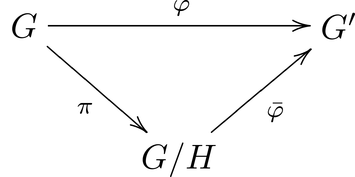
\includegraphics[width=5cm]{./factorizacion.png}
\end{figure}
Es decir, para todo $x \in G $ dicho homomorfismo cumple que $\varphi(x)=\overline{\varphi}(\pi(x))$.
\\
\\
\begin{proof}
Existencia. Sea $\varphi:G/H \rightarrow G'$ la aplicaci'on dada por $\overline{x}\rightarrow \varphi(x)$. Est'a bi'en definida porque si $\overline{x}=\overline{y}$, entonces $1=\overline{x}\overline{y}^{-1}$, con lo cual $xy^{-1}\in H \subseteq ker(\varphi)$. Por lo tanto $\varphi(xy^{-1})=1$, y entonces $\varphi(x)=\varphi(y)$. Adem'as, define un homomorfismo porque $\overline{\varphi}(\overline{xy})=\varphi(xy)=\varphi(x)\varphi(y)=\overline{\varphi}(\overline{x})\overline{\varphi}(\overline{y})$. Para ver que hace conmutar el diagrama, notar que para todo $x \in G$ se cumple $\varphi(x)=\overline{\varphi}(\overline{x})=\overline{\varphi}(\pi(x))$.\\
Unicidad. Para la unicidad, basta observar que la manera en que fue definido el homomorfismo $\overline{\varphi}$ es la 'unica manera de definirlo de tal manera que conmute con el diagrama. Es decir, si se tiene un homomorfismo $\psi$ que conmuta con el diagrama, $\psi(\overline{x})=\varphi(x)$ para todo $x \in G$, y entonces $\psi = \overline{\varphi}$.
\end{proof}

\subsection{Teoremas de isomorf'ia.}
\subsubsection{Primer teorema de isomorf'ia.}
\begin{teorema}
Sean $G$ y $G'$ grupos arbitrarios y sea $\varphi:G \rightarrow G'$ Un homomorfismo de grupos. Entonces $G/ker(\varphi)\simeq im(\varphi)$.
\end{teorema}
El simbolo $\simeq$ indica que los dos elementos son isomorfos.
\\
\\
\begin{proof}
Usando la factorizaci'on de homomorfismos de grupos sobre el n'ucleo $ker(\varphi)$, se tiene que existe un 'unico homomorfismo $\overline{\varphi}:G/ker(\varphi)\rightarrow G'$ tal que $\varphi=\overline{\varphi}\cdot\pi$.\\
Si consideramos dicho homomorfismo $\overline{\varphi}$ restringiendo su dominio a $im(\varphi)$ tendriamos un epimorfismo, porque por definici'on de la imagen, para todo $y \in im(\varphi)$ existe un $x \in G$ tal que $\varphi(x)=y$, y por lo tanto $\overline{\varphi}(\overline{x})=y$.\\
Ademas, es un monomorfismo, porque $\overline{\varphi}(\overline{x})=\varphi(x)$. Entonces si, $\overline{\varphi}(x)=0$ se tiene que $x \in ker(\varphi)$, con lo cual $\overline{x}=0$.\\
As'i, $\overline{\varphi}:G/ker(\varphi)\rightarrow im(\varphi)$ resulta un isomorfismo.
\end{proof}
\subsubsection{Segundo teorema de isomorf'ia.}
\begin{teorema}
Sean $N$ y $H$ subgrupos normales de un grupo $G$, tales que $N \subset H$. Entonces $H/N \triangleleft G/N$ y
\[
(G/N)/(H/N) \simeq G/H
\]
\end{teorema}
\begin{proof}
Consideramos la aplicaci'on 
\[
f:G/N \rightarrow G/H :aN \mapsto aH
\]
que sabemos que esta bien definida, pues si $aN = bN$, entonces $a^{-1}b \in N \subset H$, por lo que $aH=bH$.\\
Como $f((aN)(bN))=f(abN)=abH=(aH)(bH)=f(aN)f(bN)$, $f$ es homomorfismo.\\
Cada $aH \in G/H$ es $aH=f(aN)$, luego $f$ es sobreyectiva. Finalmente $aN \in ker(f)$ si y solo si $aH = f(aN)=H$, esto es,
\[
ker(f)=\{aN \in G/N\, : \, a \in H \}=H/N  
\]
Como $f$ es un homomorfismo de gupos, aplicando el primer teorema de isomorfia tenemos que
\[
(G/N)/ker(f) \simeq im(f)
\]
esto es,
\[
(G/N)/(H/N) \simeq G/H
\]
\end{proof}
\subsubsection{Tercer teorema de isomorf'ia.}
\begin{teorema}
Sean $G$ un grupo y $S$, $T$ subgrupos de $G$. Sea $S$ un subgrupo normal de $G$. Entonces se tiene que $ST/S=T/ (S \cap T)$.
\end{teorema}
\begin{proof}
Para empezar, se debe verificar que las expresiones del enunciado est'an bi'en definidas. Por un lado $ST$ es subgrupo de $G$ porque $S$ es normal en $G$. Teniendo esto en cuenta se cumple tambi'en que $S$ es subgrupo normal de $ST$, por que dado cualquier $x \in ST$, en particular $x \in G$, y por lo tanto $xSx^{-1}=S$. Por 'ultimo $S \cap T$ es subgrupo normal de $T$. Para ello, dados $t \in T$ y $s \in S \cap T$, se debe ver que $tst^{-1} \in S \cap T$. En efecto, $tst^{-1}=S$ porque $S$ es normal, y est'a en $T$ porque todos sus factores lo est'an.\\
Para el isomorfismo, vamos a considerar primero la aplicaci'on $\varphi:T \rightarrow ST/S$ definida por $t \mapsto \overline{t}=1tS$. Se tiene que $\varphi$ es un homomrfismo de grupos porque $\varphi(tt')=\overline{tt'}=\varphi(t)\varphi(t')$.\\
Por un lado, $\varphi$ es un epimorfismo. Para ver esto, considerar un elemento $stS \in ST/S$ arbitrario. Por ser $S$ normal, se sabe que $st$ se escribe como $t \widetilde s$ para alg'un $\widetilde s \in S$. Se tiene entonces que $stS=t \widetilde s S=tS=\varphi(t)$.\\
Por otro lado, el n'ucleo $ker (varphi)$ es el conjunto $\{ t \in T:tS=S \}$, es decir, $T \cap S$.\\
Resumiendo, $\varphi:T \rightarrow ST/S$ es un epimorfismo cuyo n'ucleo es $T \cap S$. Por el primer teorema de isomorfia se concluye entonces que $T/(T \cap S) \simeq ST/S$.
\end{proof}
\section{Teorema de estructura de los grupos abelianos finitos.}
El teorema de estructura de los grupos abelianos finitos constituye, por su naturaleza, una primera aproximaci'on a la clasificaci'on de los grupos, en nuestro caso de los grupos abelianos finitos.\\
Apuntemos que todo grupo c'iclico es abeliano, pero no todo grupo abeliano es ciclico, ademas, los grupos abelianos finitos son producto directo de grupos ciclicos.\\
Enunciamos a continuaci'on el teorema de estructura de los grupos abelianos finitos, del cual omitiremos su demostracion:
\begin{teorema}[Estructura de los Grupos Abelianos Finitos.]
Si $G$ es un grupo abeliano finito, existen enteros positivos $m_{1},\ldots ,m_{r}$ tales que:
\[
G \simeq Z/m_{1}Z \times \ldots \times Z/m_{r}Z
\]
y cada $m_{i}$ divide a $m_{i-1}$.
\end{teorema}
Queda claro que $o(G)=m_{1}\ldots m_{r}$. Ademas, los numeros $r, m_{1},\ldots ,m_{r}$ son 'unicos con esta propiedad. Se dice que $m_{1},\ldots ,m_{r}$ son los coficientes de torsi'on de $G$.\\
Este teorema nos permite calcular el numero de grupos abelianos finitos no isomorfos de un orden dado.\\
Pongamos un ejemplo aclarador de aplicaci'on de este teorema:\\
\\
Supongamos que deseamos calcular cuantos grupos abelianos no isomorfos existen de orden 200. El teorema de estructura reduce la cuesti'on a obtener todas las -uplas $(r,m_{1},\ldots ,m_{r})$ tales que $m_{1}\ldots m_{r}=200$ con $m_{i}$ divide a $m_{i-1}$. Asi tenemos que para:\\
\\
$r=1$:
\[
m_{1}=200
\] 
para $r=2$:
\[
m_{1}=100\, ; \,m_{2}=2
\]
\[
m_{1}=40\, ; \,m_{2}=5
\]
\[
m_{1}=20\, ; \,m_{2}=10
\]
para $r=3$:
\[
m_{1}=50\, ; \,m_{2}=2\, ; \, m_{3}=2
\]
\[
m_{1}=10\, ; \,m_{2}=10\, ; \, m_{3}=2
\]
ya no es posible encontrar mas -uplas que cumplan las condiciones del teorema. Por lo tanto hay 6 grupos abelianos, no isomorfos, de orden 200 que son:
\[
Z/200Z
\]
\[
Z/100Z \times Z/2Z
\]
\[
Z/400Z \times Z/5Z
\]
\[
Z/20Z \times Z/10Z
\]
\[
Z/500Z \times Z/2Z \times Z/2Z
\]
\[
Z/10Z \times Z/10Z \times Z/2Z
\]
por lo tanto, todos los grupos abelianos de orden 200 son isomorfos a alguno de ellos.
\section{Automorfismos de grupos.}
Los homomorfismos biyectivos de un grupo $G$ en si mismo se conocen como los automorfismos de $G$. Estas funciones conforman un grupo que tiene informaci'on importante relativa al grupo $G$.
\subsection{Automorfismos interiores.}
Veremos la relaci'on entre los automorfismos de un grupo, sus automorfismos interiores y su centro.\\
\\
Si $H$ es un subgrupo de un grupo $G$, se llama \textit{centralizador} de $H$ en $G$ a
\[
C_{G}(H)=\{ x \in G : ax = xa \,\, \forall a \in H \}
\]
Al centralizador de $G$ en $G$, simbolizado por $Z(G)$ y llamado \textit{centro} de $G$, es un grupo normal de $G$ el cual esta definido como
\[
Z(G)=\{ x \in G\, : \, xa=ax, \, \forall a \in G \}
\] 
Notese que $G$ es abeliano si y solo si $G=Z(G)$.
\begin{definicion}
Sea $G$ un grupo, un \textbf{automorfismo} de $G$ es un homomorfismo biyectivo de $G$ en si mismo. Sea $x \in G$ la funci'on definida por
\[
\phi_{x}:G \rightarrow G
\]
\[
a \mapsto x^{-1}ax
\]
es un automorfismo de $G$ y se denomina \textbf{automorfismo interior} de $G$ determinado por $x$. El conjunto de los automorfismos interiores de $G$ lo denotaremos como $Int(G)$.
\end{definicion}
Enunciamos ahora la siguiente proposici'on que nos sera de utilidad para demostrar el pr'oximo teorema:
\begin{proposicion}
Sean $G$ un grupo y $H$ un subgrupo de $G$. La aplicaci'on 
\[
\phi : N_{G}(H) \rightarrow Aut(H) \, : \, a \mapsto \phi_{a}
\]
es homomorfismo de grupos con imagen $Int(H)$ y n'ucleo $C_{G}(H)$.
\end{proposicion}
\begin{teorema}
Sea $G$ un grupo, $Aut(G)$ su colecci'on de automorfismos y sea $Int(G)$ el conjunto de automorfismos interiores de $G$. Entonces:
\begin{enumerate}
\item $Aut(G)$ es un subgrupo de grupo $S_{G}$ de funciones biyectivas de $G$ en $G$.
\item $Int(G) \triangleleft Aut(G)$
\end{enumerate}
\end{teorema}
\begin{proof}
1) La primera afirmaci'on es evidente. 2) Por comodidad, llamando $K=Int(G)$ se trata de probar, como vimos en la definici'on 1.6.1, que:
\[
K^{f} \subset K, \,\, \forall f \in Aut(G)
\]
Sea pues $g \in K^{f}$. Asi $f \circ g \circ f^{-1} \in K$, luego existe $a \in G$ tal que $f \circ g \circ f^{-1}=\phi_{a}$, donde $\phi_{a}$ es un automorfismo interior, y asi $g=f^{-1}\circ \phi_{a} \circ f$. Entonces, dado $x \in G$ y llamando $b=f^{-1}(a)$ se tiene
\[
g(x)=(f^{-1} \circ \phi_{a})(f(x))=f^{-1}(af(x)a^{-1})=bxb^{-1}=\phi_{b}(x)
\]
por tanto, $g=\phi_{b} \in K$.\\
Por 'ultimo, de la proposici'on 1.9.1 se deduce que la aplicaci'on 
\[
\phi : G \rightarrow Int(G) \,\, : a \mapsto \phi_{a}
\]
es homomorfismo sobreyectivo con n'ucleo $Z(G)$, y por ello
\[
G/Z(G) \cong Int(G)
\]
\end{proof}
\subsection{Acci'on de un grupo sobre un conjunto.}
El concepto de grupo tom'o importancia en la matem'atica cuando Lagrange y luego Galois consideraron las sustituciones de las raices de una ecuaci'on polinomial; los patrones de intercambios de las raices aportan informaci'on sobre la solubilidad de la ecuaci'on mediante f'ormulas expl'icitas. Posteriormente, Felix Klein enfatiz'o la importancia de las simetrias admisibles en la clasificaci'on de las geometrias. En los dos casos, los elementos de un grupo aparecen como transformaci'on de otros objetos (raices de una ecuaci'on algebraica; o puntos de un plano) y los objetos transformados no son menos importantes que las propias transformaciones.
\begin{definicion}
Una acci'on (a la izquierda) de un grupo $G$ sobre un conjunto $X$ es una funci'on $\phi : G \times X \rightarrow X$ tal que: 
\begin{enumerate}
\item $\phi(g, \phi(h, x))=\phi(gh, x)$ para todo $g, h \in G$, $x \in X$.
\item $\phi(1_{G},x)=x$ para todo $x \in X$.
\end{enumerate}
\end{definicion}
Se acostumbra a escribir $g \cdot x$ en lugar de $\phi(g,x)$; con esta notaci'on, las propiedades de una acci'on son:
\[
g \cdot (h \cdot x)=(gh)\cdot x
\]
\[
1_{G}\cdot x = x
\]
\begin{definicion}
Una acci'on de grupo define una relaci'on de equivalencia sobre $X$: $x\sim y$ si y solo si $x=g \cdot y$ para alg'un $g \in G$.
\end{definicion}
La \textbf{'orbita} de $x \in X$ bajo la acci'on de $G$ es la clase de equivalencia de $x$ bajo esta relaci'on:
\[
G \cdot x = \{g\cdot x \in X\, :\,g\in G \}\subseteq X
\]
Una acci'on de un grupo $G$ en un conjunto $X$ se dice que es \textit{transitiva} si para todo par de elementos $x,y \in X$ existe un $g \in G$ tal que $g \cdot x = y$. 
\begin{definicion}
Sea $\phi : G \times X \rightarrow X$ una acci'on de un grupo sobre un conjunto. El \textbf{subgrupo estabilizador} para un elemento $x \in X$ es el subgrupo
\[
G_{x}=\{g \in G\,:\,g \cdot x = x  \} \subseteq G
\]
\end{definicion}
\begin{proposicion}
Dada una acci'on de un grupo $G$ sobre un conjunto $X$, el n'umero de elementos de la 'orbita $G \cdot x$ coincide con el 'indice $[G:G_{x}]$.
\end{proposicion}
\begin{proof}
Si $h,g \in G$ y $x \in X$, entonces
\[
g \cdot x = h \cdot x \Longleftrightarrow g^{-1}h \cdot x = x \Longleftrightarrow g^{-1}h \in G_{x} \Longleftrightarrow gG_{x} = hG_{x} \in G/G_{x}
\]
luego la aplicaci'on $g \cdot x \mapsto gG_{x}$ es una biyecci'on de la 'orbita $G \cdot x$ en el conjunto cociente $G/G_{x}$. Por lo tanto $o(G \cdot x)=o(G/G_ {x})=[G:G_{x}]$
\end{proof}
\begin{definicion}
Una acci'on $\phi : G \times X \rightarrow X$ es \textbf{eficaz} (o \textbf{fiel}) si el homomorfismo $\psi : G \rightarrow S_{X}$ es inyectivo. Una acci'on es eficaz si $g \cdot x=x$ para todo $x \in X$ implica $g=1_{G}$.
\end{definicion}
Un grupo $G$ tambi'en act'ua por conjugaci'on sobre el conjunto de todos sus subgrupos, $X=\{H:H\subseteq G \}$. Esta acci'on est'a dada por la f'ormula $g \cdot H = gHg^{-1} $. La 'orbita de H bajo esta acci'on es la familia de subgrupos conjugados de $H$. \\
El subgrupo estabilizador de $H$ en este caso es el \textbf{normalizador} de $H$, definido como:
\[
N_{G}(H)=\{g \in G : gHg^{-1}=H  \}
\]
Se puede observar que $N_{G}(H)$ es un subgrupo de $G$, no necesariamente normal, pero $H$ es un subgrupo normal de 'el: $H \triangleleft N_{G}(H)$.
\subsection{Teorema de Sylow.}
Antes de enunciar los teoremas de Sylow debemos introducir el concepto de \textit{p-grupo} y el \textit{Teorema de Cauchy}.
\begin{definicion}
Sea $p$ un n'umero primo. Un grupo finito $G$ se denomina \textit{p-grupo} si $o(G)=p^{r}$, con $r \in \mathbb{Z}^{+}$.
\end{definicion}
Antes de continuar es importante destacar dos resultados que usaremos en la demostraci'on del Teorema de Syllow:
\begin{enumerate}
\item \textit{Congruencia de los puntos fijos.} Si $G$ es un \textit{p-grupo} y $G$ opera sobre un conjunto finito $X$, entonces:
\[
o(X) \equiv o(X_{0}) (mod \, p)
\]
Donde $X_{0}\subseteq X$ es el conjunto de puntos fijos, 
\[
X_{0}=\{ x \in X ; Gx = \{x \} \}
\]
\item \textit{Congruencia del normalizador.} Es un caso particular del resultado anterior. Sea $H$ un \textit{p-subgrupo} de un grupo finito $G$. Entonces:
\[
[N(H):H] \equiv [G:H] (mod \, p) 
\]
\end{enumerate}
\begin{teorema}[Teorema de Cauchy]
Sea $G$ un grupo finito de orden $n$ y $p$ un n'umero primo que divide a $n$. Entonces $G$ tiene un elemento (y por lo tanto un subgrupo) de orden $p$.
\end{teorema}
\begin{proof}
Sea $X= \{ (x_{1},\ldots ,x_{p})\in G^{p}\, : \, x_{1}\ldots x_{p}=1\}$. Si $k \in \mathbb{Z}_{p}$, la relaci'on 
\[
k(x_{1},\ldots ,x_{p})=(x_{k+1},\ldots ,x_{p},x_{1},\ldots ,x_{k})
\]
define una acci'on de $\mathbb{Z}_{p}$ en $X$. Como $\mathbb{Z}_{p}$ es un p-grupo y $o(X)=n^{p-1}$, se tiene que $o(X_{0})$ es multiplo de $p$, siendo
\[
X_{0}=\{ (x,\ldots ,x)\, : \, x \in G \, ,x^{p}=1 \}
\]
Dado que $X_{0}$ contiene el elemento $(1, 1, \ldots ,1)$, resulta que $G$ tiene un elemento de orden $p$.
\end{proof}\\
\\
Sea $G$ un grupo finito, ante el problema de estudiar los subgrupos de $G$ es natural empezar con los p-subgrupos, para cada primo $p$. El conocimiento de estos subgrupos es muy 'util para determinar la estructura de $G$. \\
Con los teoremas de Sylow podremos conocer, si, dado un grupo finito $G$ y un primo $p$ que divida a $o(G)$, si existen p-subgrupos de cualquier orden permitido por el teorema de Lagrange, cuantos hay, y que relaci'on hay entre ellos. 
\begin{teorema}[Primer teorema de Sylow]
Sea $G$ un grupo finito, $p$ un n'umero primo y $r > 0$ un n'umero entero tales que $p^{r}$ divide a $o(G)$. Entonces existen subgrupos $H_{1}, \ldots ,H_{r}$ de $G$ tales que $o(H_{i})=p^{i}$ para $i=1,\ldots ,r$ y de modo que $H_{i} \triangleleft H_{i+1}$ para $i=1,\ldots ,r-1$.
\end{teorema}
\begin{proof}
Si $r=1$ el resultado es consecuencia directa del teorema de Cauchy. Supongamos pues que $r \geq 2$. Entonces existen, por inducci'on, subgrupos $H_{1},\ldots ,H_{r-1}$ de $G$ tales que $o(H_{i}=p^{i}\,(1 \leq i \leq r-1)$ y con $H_{i}$ normal en $H_{i+1}\, (1 \leq r \leq r-2)$. Como $p$ divide a $[G:H_{r-1}]$, por la congruencia del normalizador, vemos que $p$ divide a $[N(H_{r-1}):H_{r-1}]$. Por el teorema de Cauchy el grupo cociente $N(H_{r-1})/H_{r-1}$ tiene un subgrupo $H_{r}/H_{r-1}$ de orden $p$, o lo que es lo mismo, $H_{r}$ es un subgrupo de $N(H_{r-1})$ que contiene a $H_{r-1}$ como subgrupo normal. Como $H_{r}$ tiene orden $p^{r}$, por el teorema de Lagrange, la demostraci'on es completa.
\end{proof}\\
\\
Si $p$ es un divisor del orden $n$, de un grupo finito $G$, entonces existen p-subgrupos de Sylow de $G$. Basta con observar que si $n=p^{r}m$, $m$ primo con $p$, los p-subgrupos de Sylow de $G$ son los subgrupos de orden $p^{r}$. Si $G$ posee un 'unico p-subgrupo de Sylow $H$, entonces $H \triangleleft G$.
\begin{teorema}[Segundo teorema de Sylow]
Sea $G$ un grupo finito, $H$ un p-subgrupo de $G$ y $S$ un p-subgrupo de Sylow de $G$. Entonces existe $x \in G$ tal que
\[
H \subseteq xSx^{-1}
\]
en particular, dos p-subgrupos de Sylow de $G$ son conjugados.
\end{teorema}
\begin{proof}
Consideremos la acci'on de $H$ en $X=G/S$ por traslaciones por la izquierda. Una clase $xS \in X$ es invariante por la acci'on anterior si y solo si $hxS=xS$ para todo $h \in H$, es decir, si y solo si $x^{-1}hx \in S$ para todo $h \in H$. Como esta relaci'on es equivalente a $H \subseteq xSx^{-1}$, vemos que
\[
X_{0}=\{ xS \in X \, : \, H \subseteq xSx^{-1} \}
\]
Ahora bien, como $H$ es un p-grupo y $o(X)=[G:S]$, la congruencia de puntos fijos nos da 
\[
o(X_{0}) \equiv [G:S] \, \, (mod \, p)
\]
Como $p$ no divide a $[G:S]$, concluimos que $X_{0}$ no es divisible por $p$ y por tanto que $X_{0}$ no es vac'io.
\end{proof}\\
\\
El segundo teorema de Sylow se deduce trivialmente que la condici'on de que $G$ posea un 'unico p-subgrupo de Sylow es equivalente a que $G$ posea un p-subgrupo de Sylow normal.
\begin{teorema}[Tercer teorema de Sylow]
Sea $G$ un grupo finito, y $n_{p}$ el n'umero de p-subgrupos de Sylow de $G$. Entonces $n_{p}=[G:N(S)]$, para todo p-subgrupo de Sylow $S$ de $G$. Puesto que $[G:N(S)]$ divide a $[G:S]$, en particular tenemos que $n_{p}$ divide a $[G:S]$ para todo p-subgrupo de Sylow $S$ de $G$. Por 'ultimo, se verifica que $n_{p} \equiv 1(mod \, p)$.
\end{teorema}
\begin{proof}
Por el segundo teorema de Sylow, $n_{p}$ es el cardinal de la 'orbita de un p-subgrupo de Sylow $S$ por la acci'on de $G$ (por conjugaci'on) en el conjunto de subgrupos de $G$. De ello se deduce que
\[
n_{p}=[G:N(S)]
\]
dado que el grupo estabilizador de $S$ es $N(S)$. La primera parte del enunciado se sigue de la relaci'on
\[
[G:S]=[G:N(S)][N(S):S]
\]
Sea ahora $X$ el conjunto de p-subgrupos de Sylow de $G$. Consideremos la acci'on de $S$ en $X$ por conjugaci'on. Entonces
\[
X_{0}=\{ T \in X \, : \, sTs^{-1}=T, \, \forall s \in S \} = \{T \in X \, : \, S \subseteq N(T) \}
\]
Veamos que $X_{0}=\{ S \}$. En efecto, si $T \in X_{0}$, entonces $S$ y $T$ son p-subgrupos de Sylow de $N(T)$ y $T \triangleleft N(T)$, de donde, por el segundo teorema de Sylow, $T=S$. Como $o(X)=n_{p}$ y $o(X_{0}=1$, obtenemos la congruencia enunciada usando la congruencia de puntos fijos.
\end{proof}

\end{document}
